

\subsection{Testing Data Distribution Analysis}

\textbf{Why Ensure Balanced Testing Data?}
\begin{itemize}
    \item Prevents bias toward majority classes.
    \item Ensures the model’s performance is fairly evaluated.
    \item Helps achieve reliable generalization across all sleep stages.
\end{itemize}

The figure below shows the normalized class distribution during testing. Each class maintains an equalized density, avoiding class imbalance. This confirms that the model’s evaluation is not biased toward any specific sleep stage.

\textbf{Sampling Density Plot Showing Balanced Class Distribution:}
\begin{figure}[h!]
    \centering
    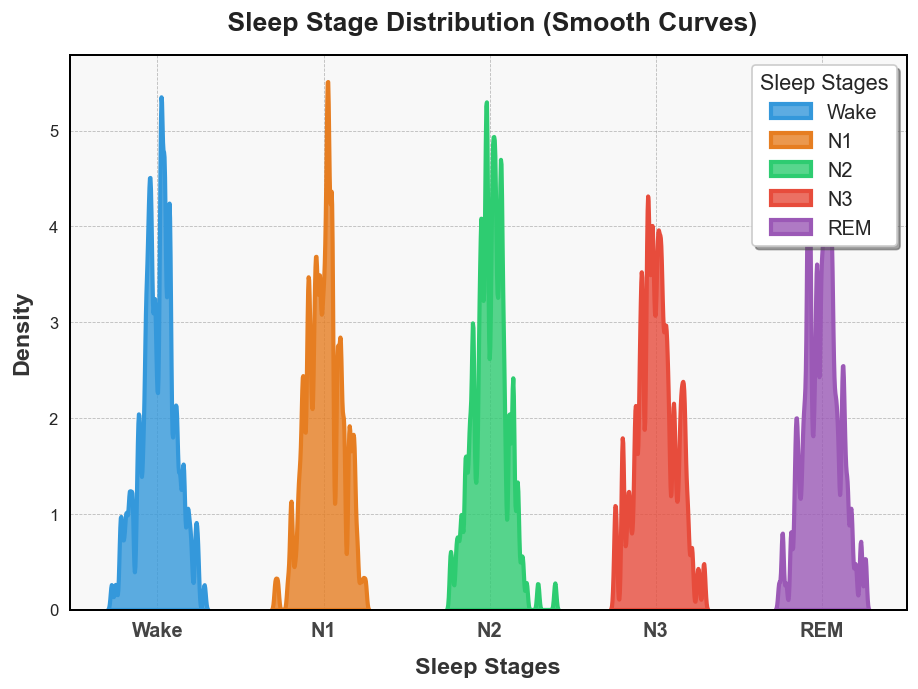
\includegraphics[width=0.8\textwidth]{img/sample distribution plot pdf.png}
    \caption{Balanced class distribution across the test set.}
\end{figure}

\subsection{Model Performance: Training vs Testing}

Figures below demonstrate the accuracy and loss curves during training and testing, providing a clear visual comparison of model performance:

\begin{figure}[h!]
    \centering
    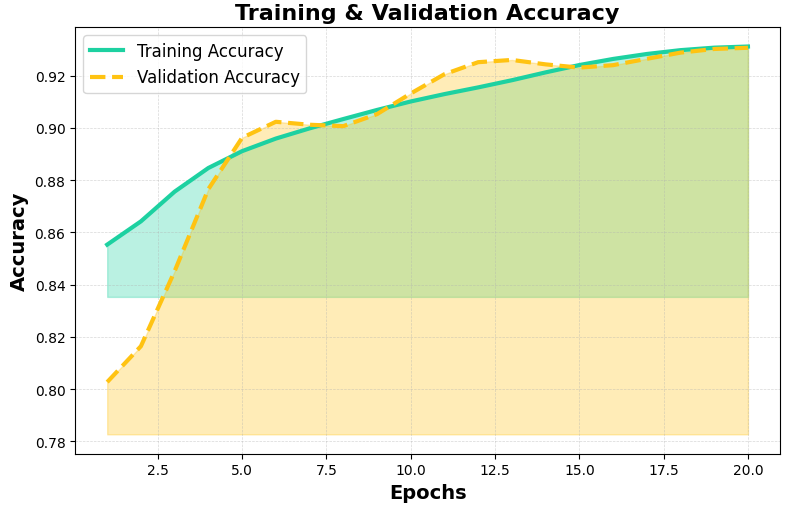
\includegraphics[width=0.8\textwidth]{img/accuracy plot.png}
    \caption{Accuracy Curve: Training vs Testing.}
\end{figure}

\begin{figure}[h!]
    \centering
    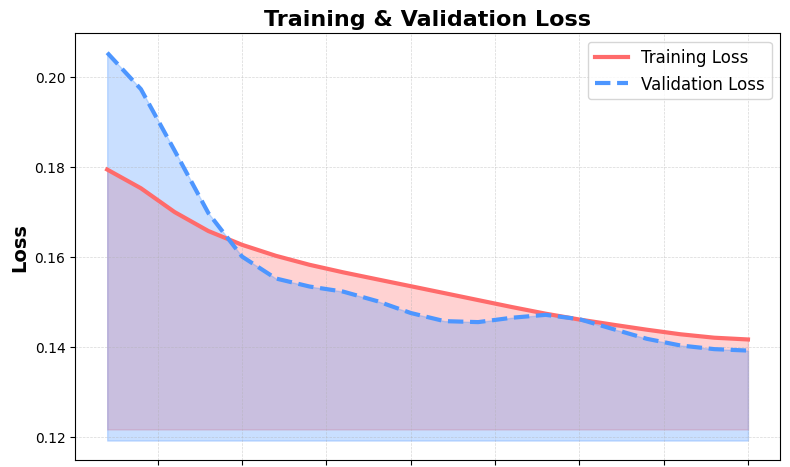
\includegraphics[width=0.8\textwidth]{img/loss plot.png}
    \caption{Loss Curve: Training vs Testing.}
\end{figure}

\subsection{Model Evaluation: Confusion Matrix}

Performance metrics are calculated to ensure a comprehensive evaluation of the model's performance across all classes. We use precision, recall, and F1-score to assess the model:

\[
\text{Precision} = \frac{TP}{TP + FP}
\]
\[
\text{Recall} = \frac{TP}{TP + FN}
\]
\[
\text{F1-Score} = \frac{2 \times \text{Precision} \times \text{Recall}}{\text{Precision} + \text{Recall}}
\]

These metrics ensure a balanced evaluation of model performance across all sleep stages.

\begin{figure}[h!]
    \centering
    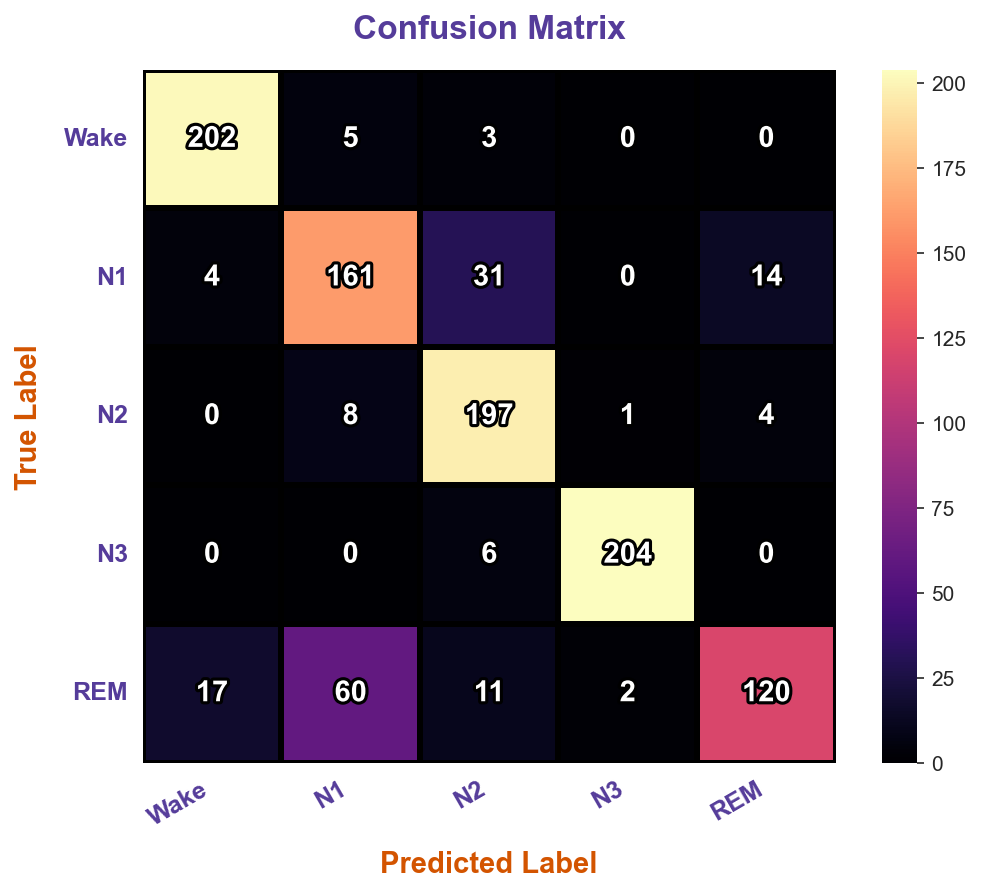
\includegraphics[width=0.8\textwidth]{img/confusion matrix samples.png}
    \caption{Confusion Matrix showing model performance across sleep stages.}
\end{figure}

\subsection{Gradient Analysis: Training Progression}

Understanding model training dynamics:

\textbf{Early Training (Epochs 0-5):} High loss with accuracy starting to improve.  
\textbf{Mid Training (Epochs 5-15):} Loss steadily decreases with stable gradient flow.  
\textbf{Late Training (Epochs 15-20):} Accuracy plateaus with no severe overfitting.

\textbf{Conclusion:} The training process remains stable, with no vanishing or exploding gradients.

\begin{figure}[h!]
    \centering
    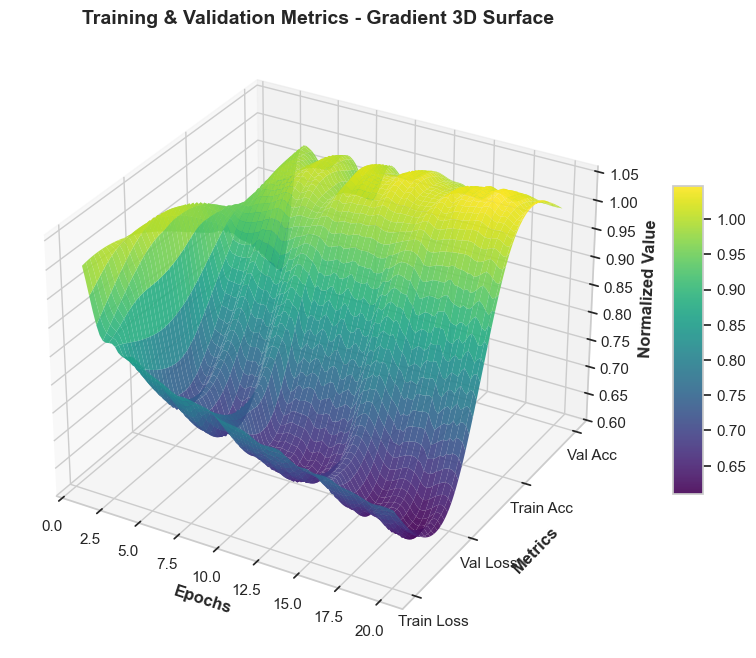
\includegraphics[width=0.8\textwidth]{img/3d gradient.png}
    \caption{Gradient 3D Surface: Training vs Validation Metrics.}
\end{figure}

\subsection{Performance Metrics: Precision, Recall, F1-Score}

Evaluating model performance across all classes using key metrics:

\begin{figure}[h!]
    \centering
    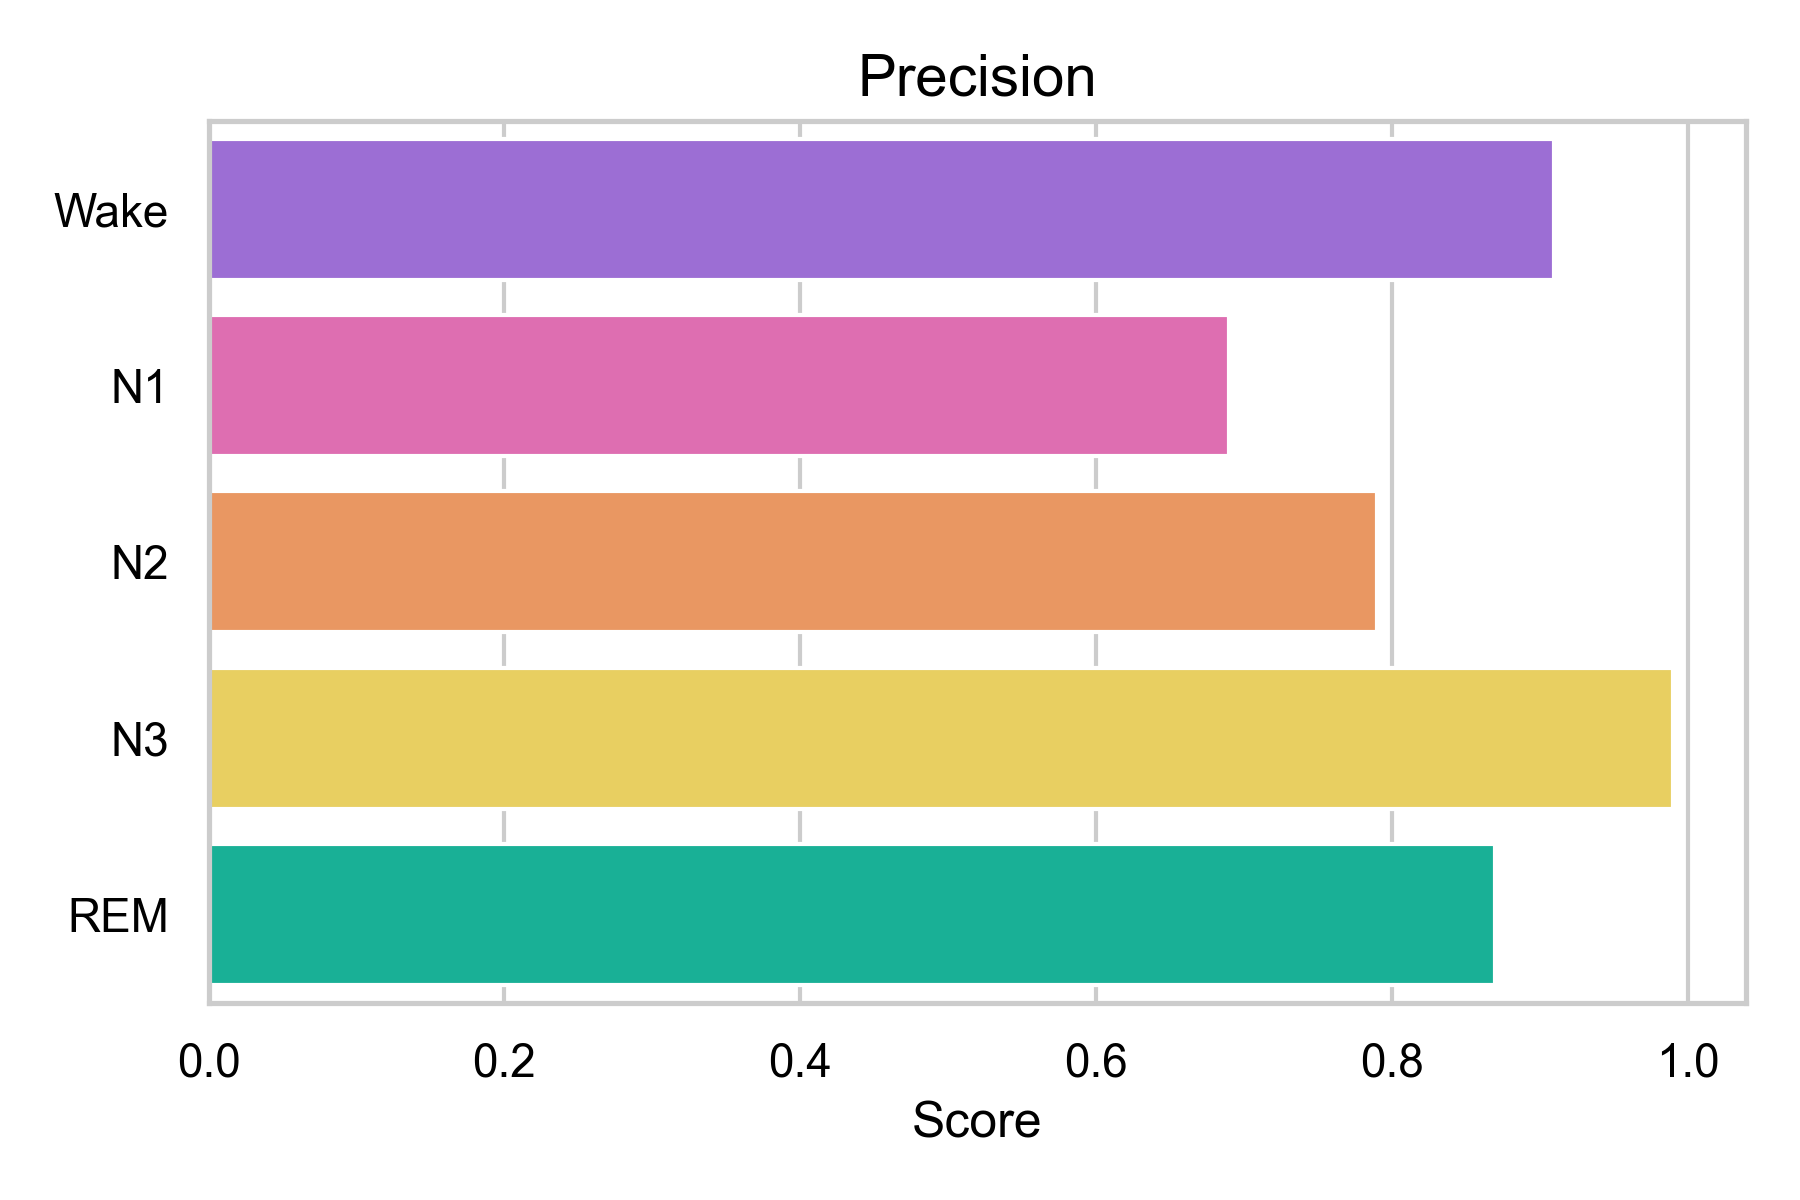
\includegraphics[width=0.8\textwidth]{img/precision_plot.png}
    \caption{Precision Scores per Class.}
\end{figure}

\begin{figure}[h!]
    \centering
    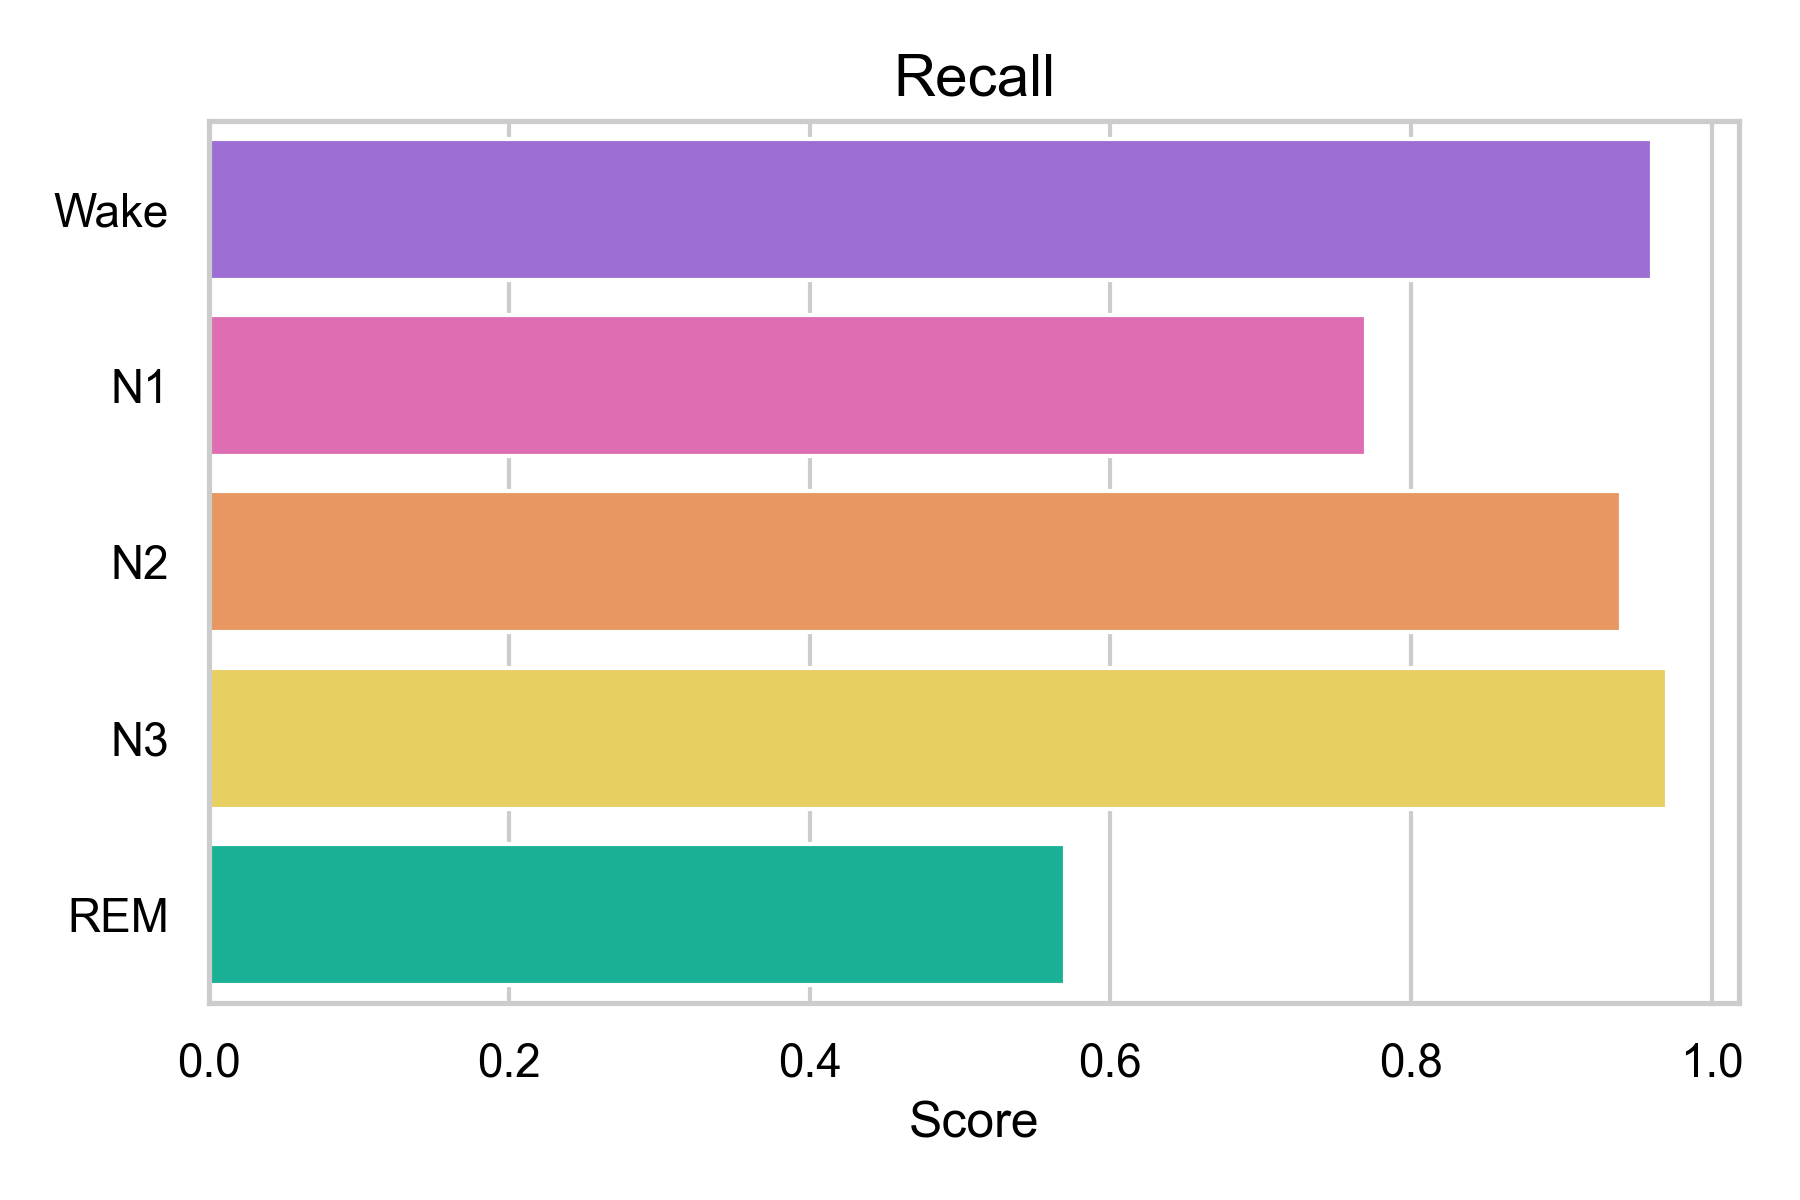
\includegraphics[width=0.8\textwidth]{img/recall_plot.png}
    \caption{Recall Scores per Class.}
\end{figure}

\begin{figure}[h!]
    \centering
    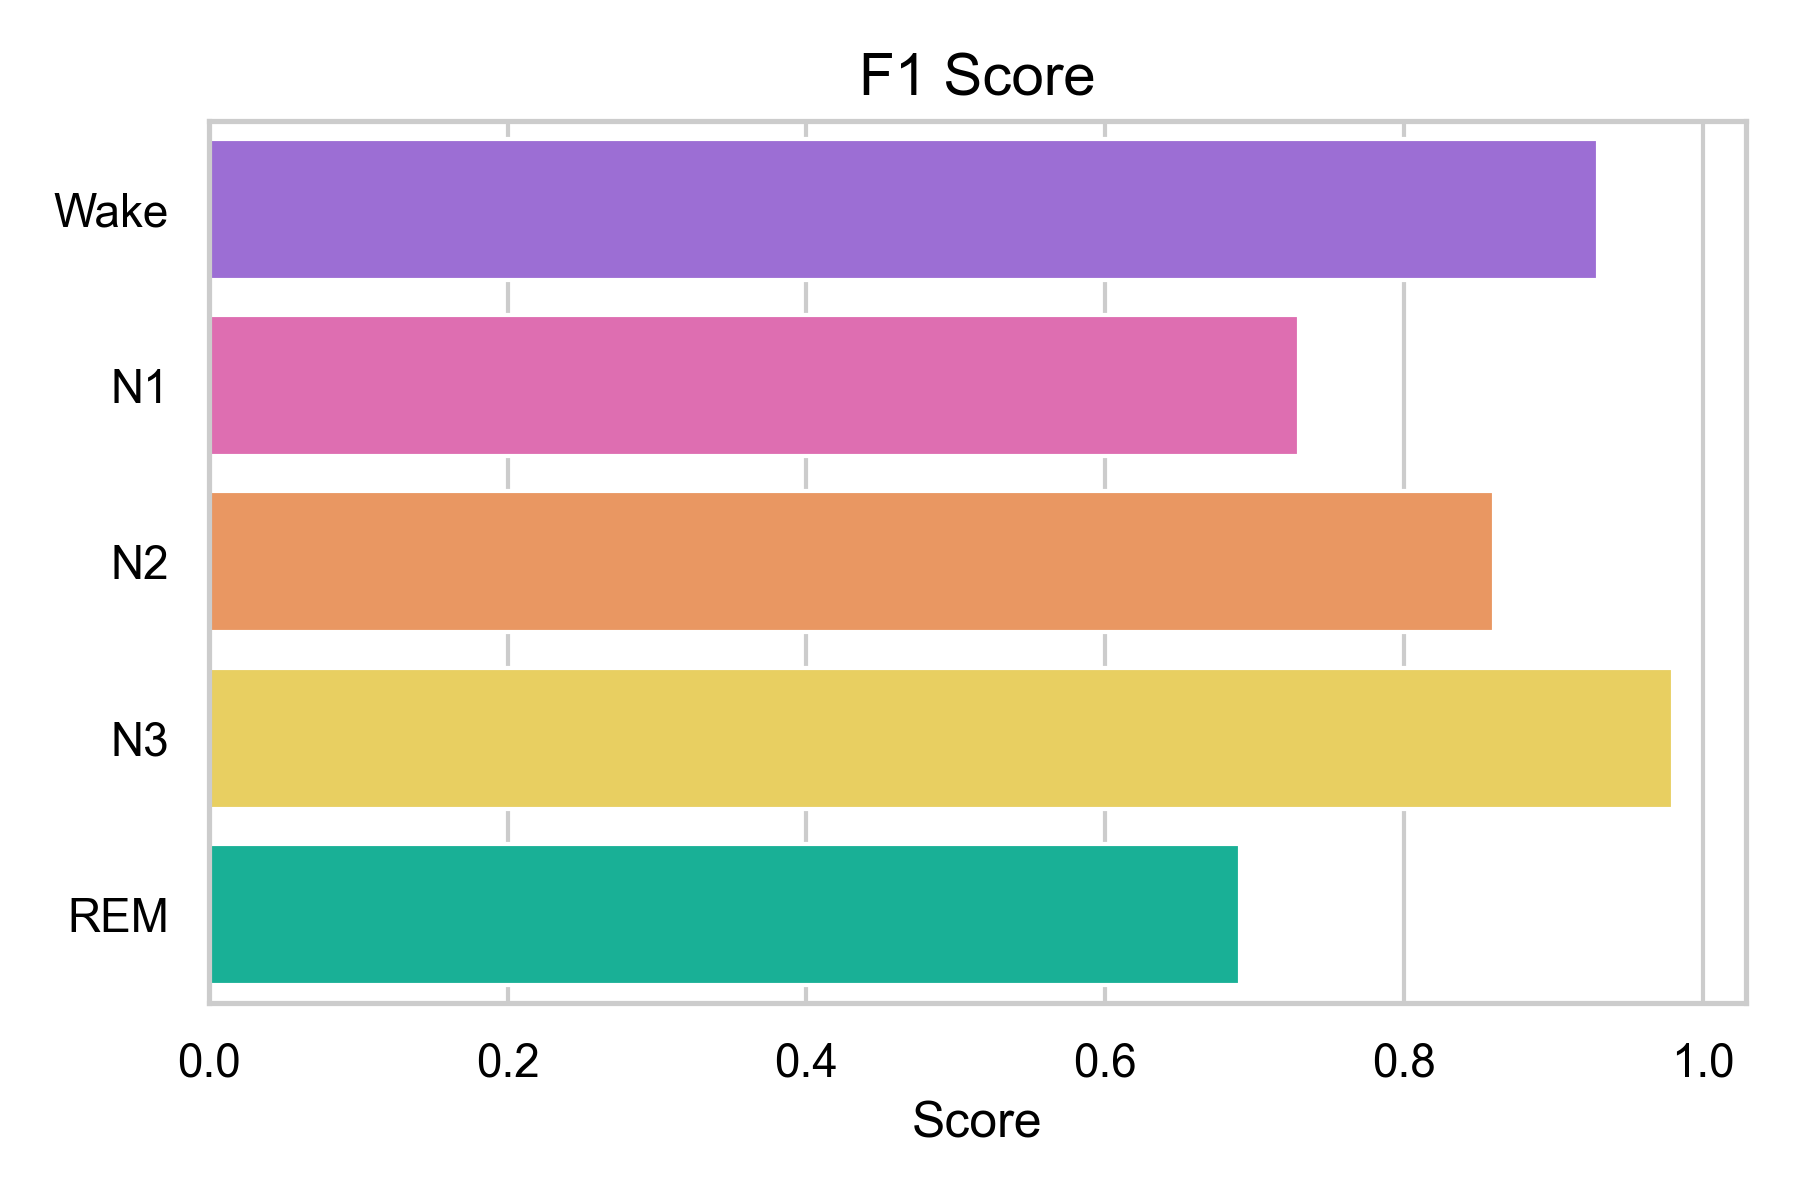
\includegraphics[width=0.8\textwidth]{img/f1_score_plot.png}
    \caption{F1 Scores per Class.}
\end{figure}

\subsection{Feature Importance Analysis with LIME}

Understanding the contribution of different channels to model predictions, we used LIME (Local Interpretable Model-agnostic Explanations) to analyze feature importance. The analysis showed that the \textbf{EMG submental} and \textbf{EEG Pz-Oz} channels contribute the most to predictions, while the \textbf{EOG horizontal} channel has minimal importance, indicating lower relevance for classification.

This insight helps optimize feature selection and improve model efficiency.

\begin{figure}[h!]
    \centering
    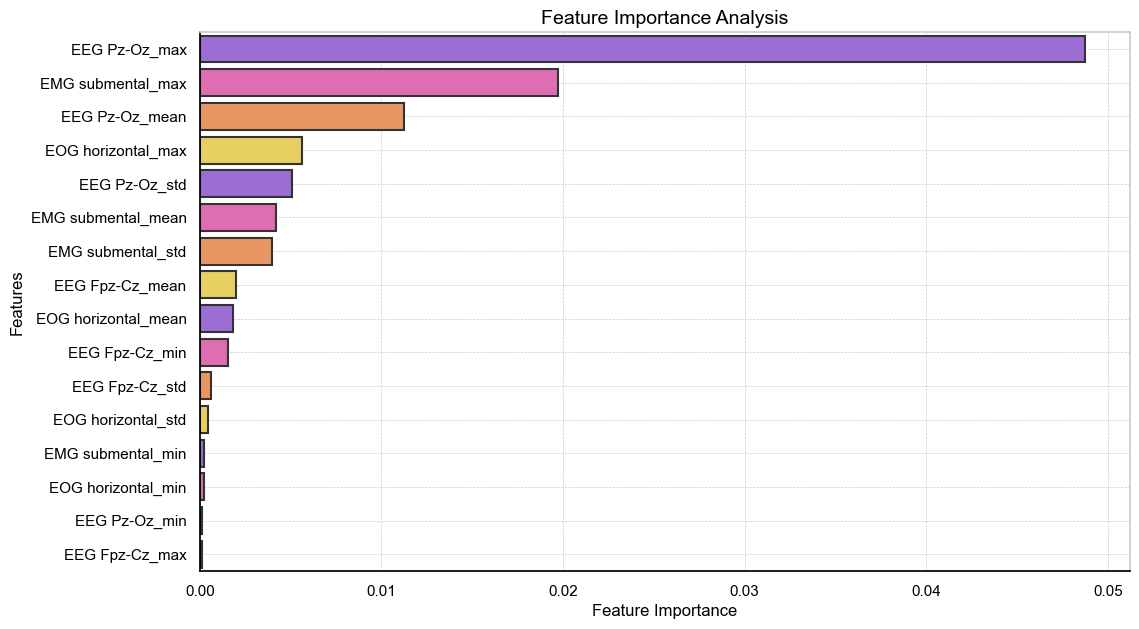
\includegraphics[width=0.8\textwidth]{img/feature importance chanels analysis.png}
    \caption{Feature Importance Analysis for 4 Channels.}
\end{figure}
